%++++++++++++++++++++++++++++++++++++++++
% Don't modify this section unless you know what you're doing!
\documentclass[letterpaper,12pt]{article}
\usepackage{float}
\usepackage[spanish]{babel}
\selectlanguage{spanish}
\usepackage[utf8]{inputenc}
\usepackage{tabularx} % extra features for tabular environment
\usepackage{amsmath}  % improve math presentation
\usepackage{graphicx, wrapfig, subcaption, setspace, booktabs}
\usepackage{graphicx} % takes care of graphic including machinery

\usepackage[margin=1in,letterpaper]{geometry} % decreases margins
\usepackage{cite} % takes care of citations
\usepackage[final]{hyperref} % adds hyper links inside the generated pdf file
\usepackage{amsmath}
\usepackage{amssymb}
\usepackage{enumerate}
\usepackage{url}
\hypersetup{
	colorlinks=true,       % false: boxed links; true: colored links
	linkcolor=blue,        % color of internal links
	citecolor=blue,        % color of links to bibliography
	filecolor=magenta,     % color of file links
	urlcolor=blue         
}
%++++++++++++++++++++++++++++++++++++++++


\begin{document}

\title{Reporte de la actividad 4}
\author{Daniela Olmos Velderrain\\Grupo 3}
\date{17 de febrero de 2019}

\maketitle

\section{Introducción}

En la actividad pasada se aplicó el uso de la biblioteca Pandas para análisis de datos sobre el regístro meteorológico de Cajeme en las últimas décadas. En esta actividad se continuará trabajando con los mismos datos de precipitación, temperaturas máximas y mínimas, pero ahora utilizaremos una nueva herramienta para visualizar los datos: Matplotlib. 
\\
\\
Mediante Matpoltlib se elaborarán diversas gráficas para representar los datos de temperaturas y precipitación obtenidos mensual y anualmente.

\section{Desarrollo}
\subsection{Metodología} 
Se importaron las siguientes librerías en el archivo de Jupyter Notebook para trabajar con los datos de Cajeme:

\begin{verbatim}
import pandas as pd
import numpy as np
import matplotlib.pyplot as plt
import calendar
import seaborn as sns
\end{verbatim}

Estas nos ayudarán con los cálculos matemáticos, el análisis estadístico y la realización de gráficas.

Para evitar los valores nulos, se les asignó a estos una variable:

\begin{verbatim}
sentinels = {'PRECIP': ['Nulo'],'EVAP':['Nulo'],'TMAX':['Nulo'],'TMIN':['Nulo']}
\end{verbatim} 

Después se leyó el archivo mediante el comando "pd.read\_csv" (indicando con na\_values=sentinels que los valores en dicha variable son datos nulos), y posteriormente se creó un Data Frame mediante el comando "pd.DataFrame()".

Como el archivo cuenta con una columna de fechas, a esta se le dio formato de fecha mediante:
\begin{verbatim}
    df['FECHAN'] = pd.to_datetime(df.apply(lambda x: x['FECHA'], 1), dayfirst=True)
    
    df = df.drop(['FECHA'], 1)
\end{verbatim}

Para poder definir columnas para meses y años, estos se extrajeron de la nueva variable "FECHAN".

\begin{verbatim}
df['MES'] = df['FECHAN'].dt.month
df['AÑO'] = df['FECHAN'].dt.year
\end{verbatim} 

Para averiguar el número de años que hay en el archivo, se contaron los datos diferentes de esta columna, obtenienedo 32 años, los cuales se guardaron en la variable "NumA":
\begin{verbatim}
NumA = len(df['AÑO'].unique())
\end{verbatim} 

Para tener arreglos con años y meses se llenaron dos vectores mediante loops, el de los años de 0 a NumA, y el de los meses de 0 a 12. Para tener los nombres de los meses, también se creó un arreglo, utilizando la biblioteca "calendar":
\begin{verbatim}
init = 1980
AÑOS = [init + i for i in range(0, NumA)]
init2 = 1
MESES = [init2 + i for i in range(0, 12)]
MESESlabel = calendar.month_name[1:13]
\end{verbatim} 

Estos arreglos servirán de etiquetas en el eje x más adelante.

Ahora, para calcular el promedio mensual de temperaturas y precipitaciones se crearon tres arreglos distintos, los cuales extraen información del DataFrame:
\begin{verbatim}
PRECIPPROPMES = [df[df.MES==(init2 + i)].PRECIP.sum()/NumA for i in range (0,12)]
TMAXPROMMES = [df[df.MES==(init2 + i)].TMAX.mean() for i in range (0,12)]
TMINPROMMES = [df[df.MES==(init2 + i)].TMIN.mean() for i in range (0,12)]
\end{verbatim} 

Este mismo procedimiento se siguió para los datos anuales, pero ahora con la columna 'AÑOS'.
\\
\\
Los arreglos realizados se utilizaron para hacer las gráficas de barras y de evolución.
\\
\\
Las gráficas de barras se realizaron de la siguiente manera:
\begin{verbatim}
X = MESESlabel
N = np.arange(len(X))
Y = PRECIPPROPMES 
 
plt.bar(N, Y,  width=0.5,align='center', alpha=0.7,color='b')
plt.xticks(N, X, size = 'small', color = 'k', rotation = 90)
\end{verbatim} 
Se llevó a cabo el mismo procedimiento para la gráfica de años.
\\
\\
Para la gráfica de evolución se realizaron dos gráficas en la misma figura, y así poder comparar la temperatura mínima y máxima a través del tiempo.
\begin{verbatim}
X = AÑOS
N = np.arange(len(X))
Y1 = TMINPROMAÑO
Y2 = TMAXPROMAÑO
 
plt.plot(Y1, label = "Temperatura mínima", color = 'y')   
plt.plot(Y2, label = "Temperatura máxima", color = 'b')
plt.xticks(N, X, size = 'small', color = 'k', rotation = 90)
\end{verbatim}
\\
\\
Para hacer los gráficos de caja se recurrió a la biblioteca Seaborn, ya que no fue posible realizarla mediante Matplotlib.
Se recurrió a los siguientes comandos para hacerlo a partir del DataFrame:

\begin{verbatim}
box = sns.boxplot(x="MES", y="TMAX", data=df)
box.set( xlabel= 'Meses', ylabel= 'Temperatura máxima (°C)')
box.set_xticklabels(MESESlabel, rotation=90 )
\end{verbatim}

\subsection{Resultados}
Las gráficas resultantes fueron las siguientes:

\begin{figure}[H]
\centering
\fbox{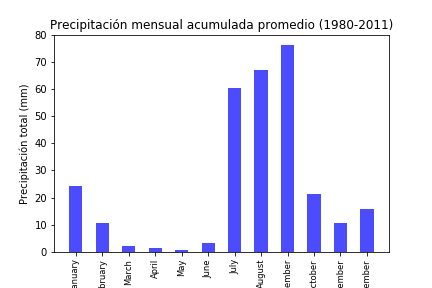
\includegraphics[width=0.5\linewidth]{Precip_mensual.png}}
\label{fig:esquema1}
\end{figure}
De acuerdo a la gráfica, la mayoría de las precipitaciones suelen encontrarse en los meses de julio, agosto y septiembre.
\\
\\
\begin{figure}[H]
\centering
\fbox{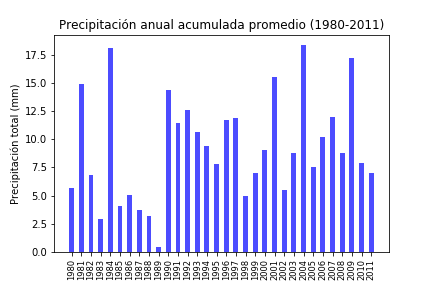
\includegraphics[width=0.5\linewidth]{Precip_anual.png}}
\label{fig:esquema2}
\end{figure}
En esta gráfica se puede observar la precipitación promedio por año, destacando que las lluvias han aumentado en las últimas décadas.
\\
\\
\begin{figure}[H]
\centering
\fbox{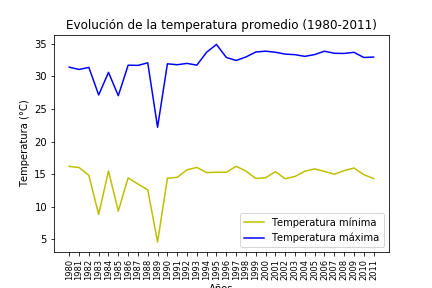
\includegraphics[width=0.5\linewidth]{Temp_anual.png}}
\label{fig:esquema3}
\end{figure}
Mediante esta gráfica podemos observar el progreso de las temperaturas a lo largo del año. Como se puede ver, estas avanzan de manera equidistantes entre ellas. 
\\
\\
\begin{center}
	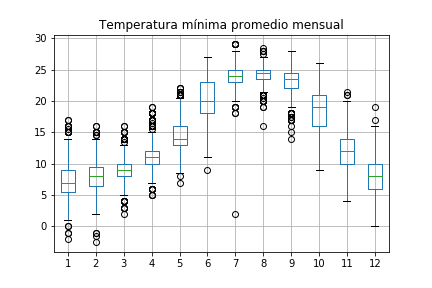
\includegraphics[height=5cm]{cajamin_mensual2.png} \hspace*{\fill}
    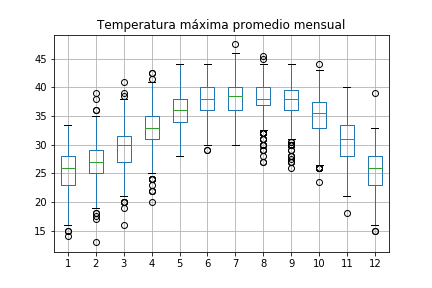
\includegraphics[height=5cm]{cajamax_mensual2.png}
\end{center}
En estas gráficas se puede observar cómo las temperaturas mínimas y máximas parecen seguir el mismo patrón, siendo estas mayores en los meses de verano y menores en lo meses invernales.
\\ 
\\
\begin{center}
	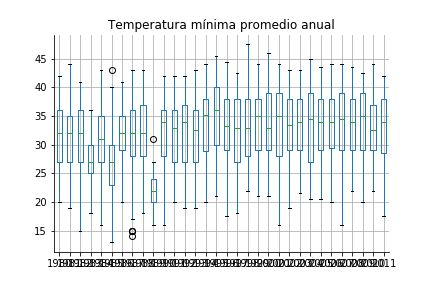
\includegraphics[height=5cm]{cajamin_anual2.png} \hspace*{\fill}
    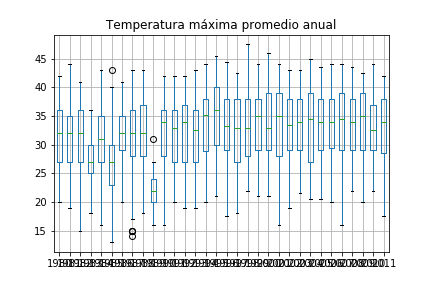
\includegraphics[height=5cm]{cajamax_anual2.png}
\end{center}
En estas gráficas se muestran los diagramas de caja de la temperatura a través de los años, tanto de temperatura mínima como máxima por separado. 

\section{Conclusiones}
La biblioteca Matplotlib es una herramienta muy útil para visualizar datos y realizar un análisis de los mismos. La visualización es un aspecto importante para evaluar datos a simple vista, ya que nos facilita la interpretación de los resultados obtenidos, más cuando hay gran cantidad valores qué analizar como en el caso de los datos meteorológicos. 

\section*{Bibliografía}
\begin{itemize}
\item \\Matplotlib. Recuperado el 17 de febrero de 2019 desde \\https://matplotlib.org/
\item Boxplot. seaborn.pydata.org. Recuperado el 17 de febrero desde\\       https://seaborn.pydata.org/generated/seaborn.boxplot.html
\end{itemize}


\end{document}